\documentclass[12pt,aps]{revtex4}
\usepackage{graphicx}
\def\thesection{}
\def\thesubsection{S\arabic{subsection}}
\renewcommand{\thefigure}{S\arabic{figure}}
\renewcommand{\thetable}{S\arabic{table}}
\renewcommand*{\citenumfont}[1]{S#1}
\renewcommand*{\bibnumfmt}[1]{[S#1]}
\begin{document}
%\title{Supplement materials to manuscript ''Declination of opinions in modern molecular biology''}
%\author{Sergey Feranchuk}
%\maketitle

\section{Computational methods}

\subsection{Human evolution}

The size of simulated ''genome'' was 1000 ''residues''. Two distributions of mutation rates across genome were used, with the same average rate $r_0$. A continuous distribution $r_c$ did depend from a genome position $x$ as $r_c(x) = A / ( x + x_0 )$, $A$ and $x_0$ were chosen so that $r_c(1) = 1$. The two-modal distribution $r_d$ was $r_d(x) = A \theta( x - x_0 ) + B$,  $A$, $B$ and $x_0$ were chosen so that $r_c(1) = 5 r_0$, $\theta$ is the ''theta-function''. 

In all kinds of analysis, the diploid data was reduced to a single sequence, the dot symbol ('.') was inserted in a position of SNP in a case of ambiguity.

MSMC binary, version 1.1, which was used in the comparative tests, was downloaded from \textit{Github} site. VCF files, which ere processed to present an analysis of human genetic data, were downloaded from \textit{1000 genomes} project site. The data in VCF files was filtered to leave only those SNPs which are used in the genotyping in the \textit{Family Tree DNA} service.

The simplest distance-based clustering, which is also known as UPGMA method or clustering with ''weighted average'', was chosen to represent distance-based methods. A distance to ambiguous positions was taken 1/2 when compared to a definite nucleotide, and 1 when compared to another ambiguous site. 

No sensitivity to ''over-dispersion'' was observed for UPGMA cluster method. An ability to reconstruct variations of population size is one of the advantages of MSMC approach, but this feature lost a stability in the tests with perturbations, so the simple distance-based clustering appeared to be competitive to be applied to a human genome data.

\begin{figure}[h]
\centerline{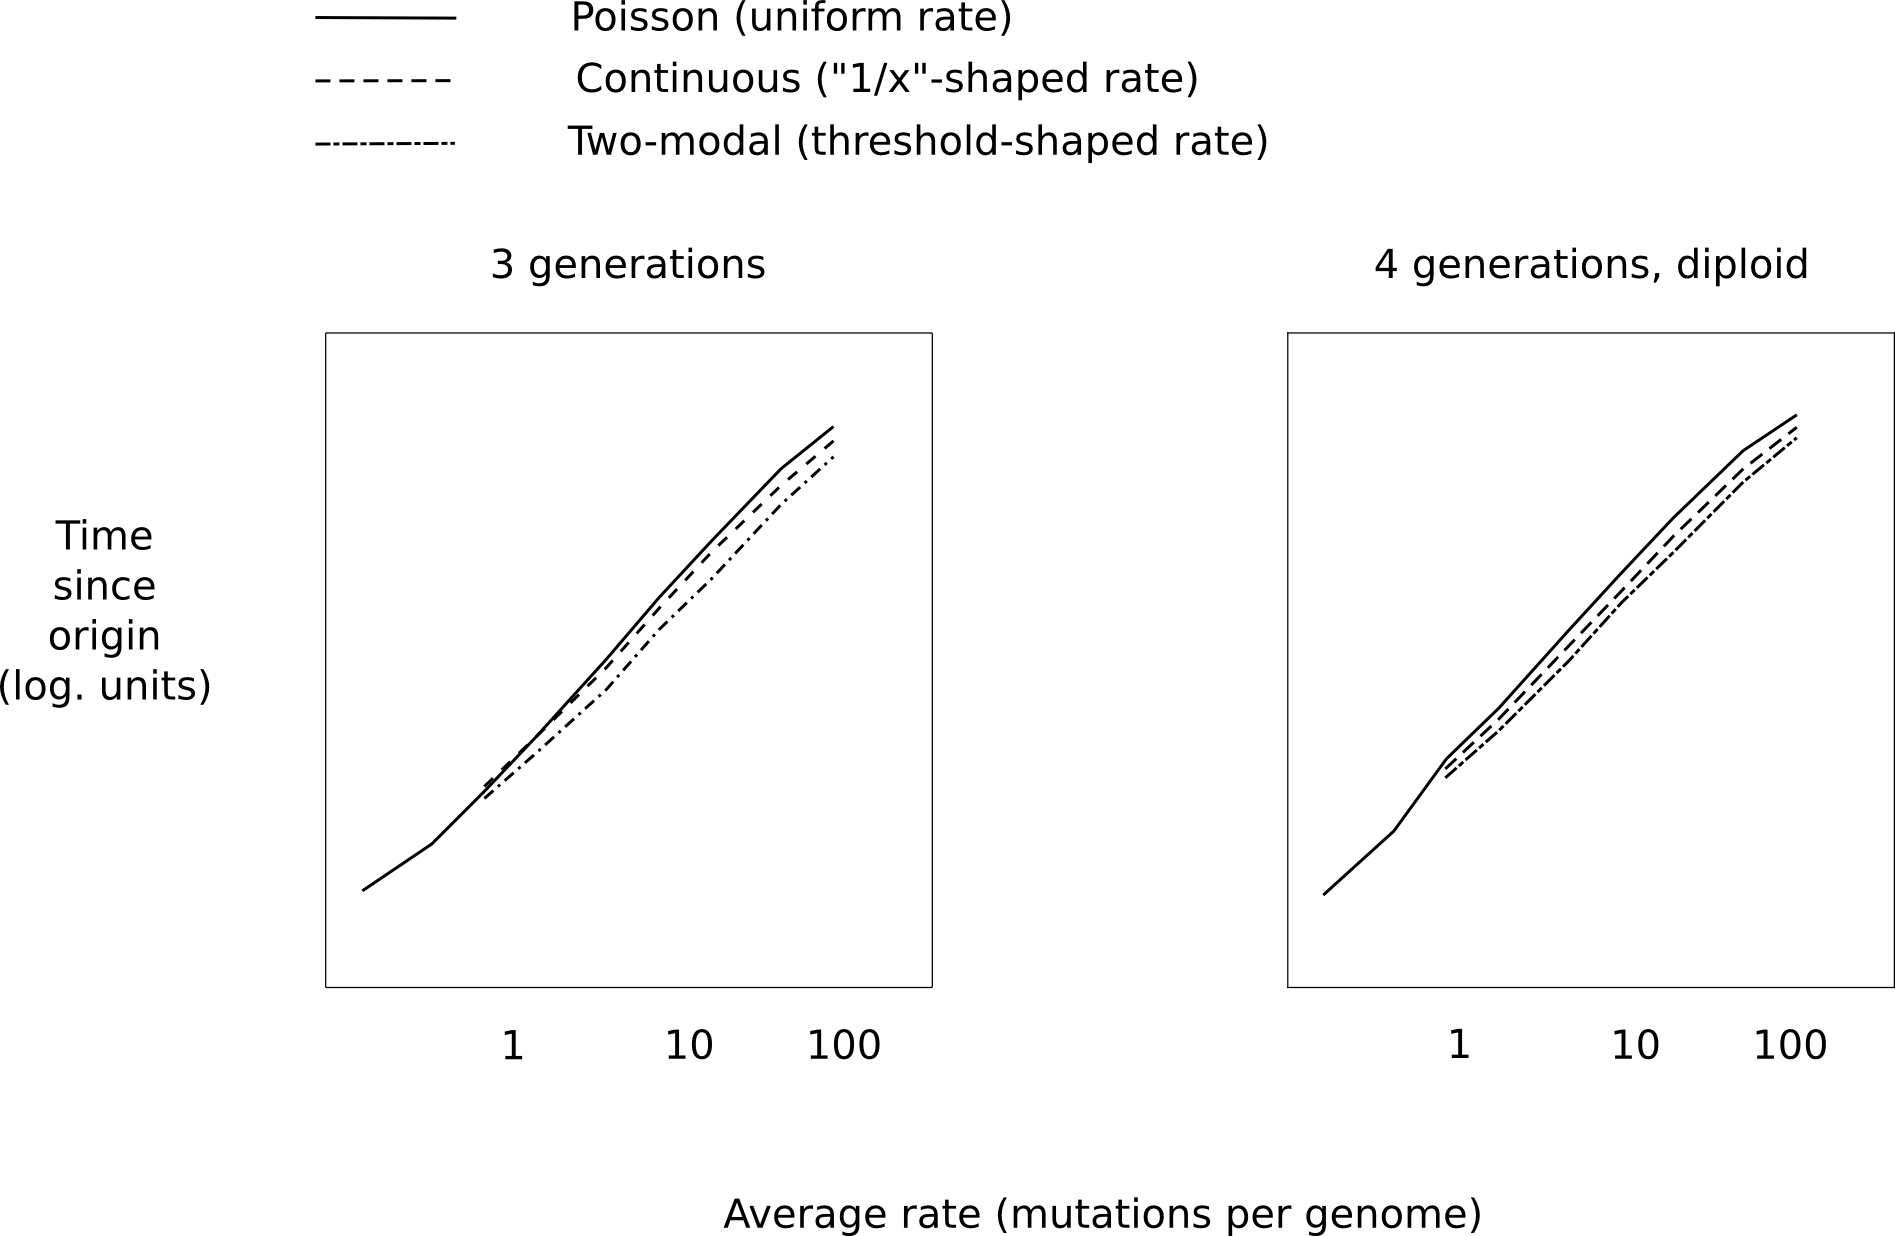
\includegraphics[width=0.8\columnwidth]{fig_upgma.png}}
\caption{Performance of UPGMA distance-based clustering on the two series of simulated genomes. A depth of a constructed tree is plotted against an average mutation rate, for the same three types of distribution as in the tests of MSMC.}
\label{fig_upgma}
\end{figure}

The distance-based UPGMA tree for human evolution was from SNPs which were extracted from VCF files on \textit{1000 genomes} project site. The distortion of historic time is a weakness of distance-based methods, but relative positions of diverged nodes continue to make sense in that trees. A period of human expansion is clearly detected on the reconstructed tree. It is almost the same for all ethnic groups, and its positioning in historic time is fit to known time of the expansion. 

683374 SNPs were taken for the analysis, from about 3 millions. The size of human genome is around $3 \times 10^9$. The position on the fig. 7A which corresponds to a beginning of human expansion is around 0.6 of the total number of SNPs. The estimates of a mutation rate in autosomal part of human genome differ between each other, but all of it are of order $10^{-9} - 10^{-10}$ per year. This is in a qualitative agreement with a a value of 50000 years for the estimated beginning of expansion. 

\subsection{RNA-seq}

Comparison of the texts was perfomed as follows:

\begin{itemize}

\item The texts of manuscripts were cleaned from auxiliary information, so that just a continuing narrative left, from Introduction to Discussion parts. Then the texts were split to words and the list of words was divided to seven equal parts.

\item The ''meaningful'' words were selected as the words which repeat in the adjacent sentences, so that it can be a subject of narrative or have some importance to it. The most common words of the language, \textit{the}, \textit{a}, \textit{of}, \textit{and}, \textit{or}, \textit{in}, were filtered, but the words \textit{we}, \textit{this}, \textit{to}, \textit{that}, \textit{as}, \textit{which},  \textit{be}, \textit{for}, \textit{period} are mostly auxiliary but it's presence or absence can be a specific feature of a fragment of text.

\item A number of ''meaningful'' words common to fragments of both texts were shown in a simulation of correlation map. The increase of a number of common words to the ending of both text is interpreted as due to presence of common rules in which a narrative in both texts is developing.

\end{itemize}

The surveys which were used to prepare a PCA charts are listed in table S1.  \textit{Illumina HiSeq 2000} sequencing with single-end reads was used in all three surveys.

\begin{table}[h] \label{table1}
\begin{center}
\begin{tabular} {|c|c|c|}
\hline
Project ID&Number of samples&Deposition date\\
\hline
PRJNA236322&59&01/23/14 (1)\\
PRJNA258388&124&08/18/14 (1)\\
PRJNA275921&60&02/20/15 (2)\\
\hline
\end{tabular}
\end{center}
{\small Deposited by: (1) Yanai, Biology, Technion - Israel Institute of Technology;
(2) University of Queensland.} 
\end{table}

Coding sequences of genes were used to estimate levels of gene expression from the transcriptome sequencing. To do this, raw archives of reads were downloaded from \textit{NCBI} and pre-processed using \textit{Trimmomatic} software. After that, the reads were aligned to Aqu2 version of \textit{A.queenslandica} genome with \textit{bowtie2} and a median coverage of each gene sequence was transformed to a level of expression. 

In order to generate an array of loosely bounded groups of genes, a network of gene interactions was reconstructed based on the estimated levels of gene expression. Edges in the network were assigned if a value of correlation between genes was above 0.7.  Kendall rank correlation was applied there, for all the samples from the three surveys. To generate 1000 groups of genes,  a sub-network of a randomly selected genes was separated each time, and a combination of community detection algorithms from \textit{igraph} software library was applied to this sub-network. In the result, the sizes of obtained groups were around $16$, and strictly within interval $16 \pm 1$.

The two of generated groups which are better separate development stages where selected to demonstrate ability to reduce a separation of development stages to a small number of genes. PCA decomposition implemented in \textit{sklearn} library and \textit{Permanova} algorithm from \textit{skbio} library were used to re-evaluate and demonstrate the efficiency of the separation, which is of order $e^{-6}$ for the selected groups.

\subsection{Re-evaluation of CASP targets}

Protein structures were analyzed which were presented as targets in 11 rounds of CASP, from 2 to 13. Four types of metrics were used to assess a complexity of a structure are specified below: 

\begin{enumerate}
\item $6 \times 6$ square slices of a binary contact map; 
\item distances in triangles of contacting residues, split to 2 bins; 
\item distances from 2 to 10 A, split to 32 bins; 
\item distances from 2 to 10 A, in the nodes of 6x6 square in contact map, split to 8 bins. 
\end{enumerate}

The processing of a whole protein chain applying any of the metrics provides a set of binary distributions and averaged values in each bin of a distribution were than converted to entropy measure. This value of entropy provided an estimate of a complexity of the structure. The properties of each metrics are provided below.

\begin{center} 
\begin{tabular} {|l|cccc|}
\hline
\textbf{Metrics} & 1 & 2 & 3 & 4 \\
\hline
number of bins & 36 & 7 & 32 & 32 \\
threshold (in angstroms) & $<$ 6 &  $<$ 8 & 2 to 10 & 2 to 10 \\
\hline
Average enthropy: & & & & \\
CASP targets & 3.58349 & 1.447 & 3.097 & 3.127 \\
subsample of PDB & 3.58350 & 1.497 & 3.146 & 3.167 \\
\hline
\end{tabular}
\end{center}

The structures of CASP targets were used in the analysis, which were opened after the rounds were finished. In earlier rounds of CASP the identifiers of structures are available in the official site. For rounds from 11 to 13, \textit{blastp} search in \textit{pdbaa} blast database was applied to get the identifiers of structures with a complete identity with the target sequences. A total number of structures to be processed was 790.

To estimate an average complexity of the structures in the protein databank (PDB), a set of 1000 non-redundant protein structures was selected from PDB. It was composed from representatives of protein clusters with 30\% identity available in \textit{RCSB} site, 100 structures were taken for each two-year period from 2000 to 2020.

\subsection{Re-evaluation of publication activity}

In publications \cite{CM1,CM2,CM3,CM4,CM5,CM6,CM7} genes considered important for the treatment of oncology diseases, are extensively studied. These seven genes were selected to make up a first list. A second list of genes was selected from the mentioned review of Morris and Chan, the only filter in the selection was to avoid terms which had some ambiguity.

The total number of publications where any of the selected genes was mentioned, was obtained by a straightforward text search in the \textit{NCBI} databank. The \textit{biopython} library was used to access it through the \textit{Entrez} interface.

In order to follow the ''econophysics'' model, the distributions of the numbers obtained needed to be converted to a uniform measure of fitness to a probability distribution, thus making it possible to choose between Pareto distribution and exponential distribution. The method which was used to measure the fitness of a random subsample to a pre-defined probability distribution, is explained in fig. \ref{onco_entropyscheme}.

\begin{figure}[h]
\centerline{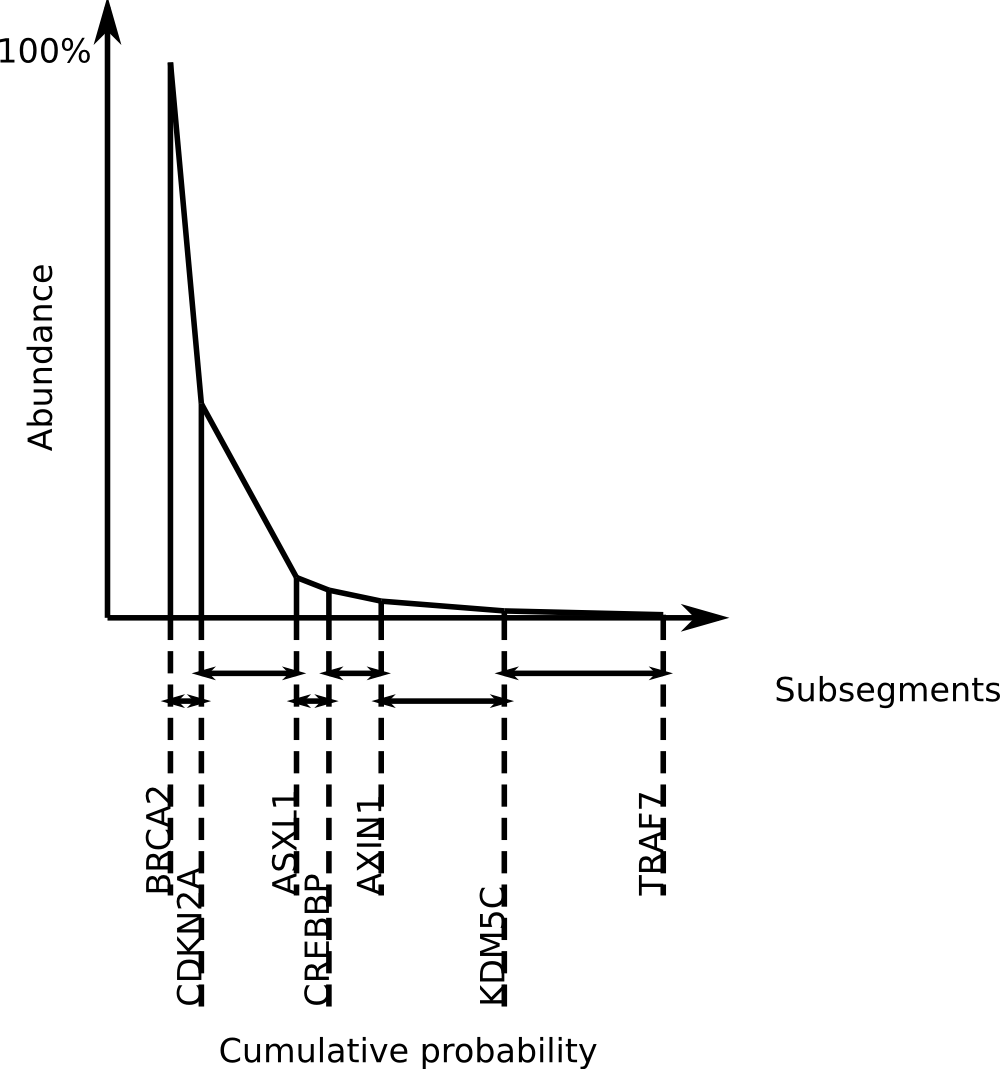
\includegraphics[width=0.7\columnwidth]{onco_entropyscheme.png}}
\caption{Illustrates the method of estimating the entropy measure, as a criteria of fitness to a probability distribution. The uneven levels of abundances (Y axis) are transformed to a more flat separation of segments (X axis) following the chosen shape of the distribution.}
\label{onco_entropyscheme}
\end{figure}

In the case of a uniform distribution, the entropy for a random subsample should be higher than for any subsamples not selected randomly, and therefore following some another trend. In this way the degree of evenness in the separation of the segments shown in fig. \ref{onco_entropyscheme} was converted to the entropy measure. Both Pareto distribution and exponential distribution are described by a single parameter, and, in both cases, an optimal value of the parameter can easily be found by a maximal likelihood criterion. The distributions fit the data better when the measured numbers or abundances are transformed to a flatter separation of segments.

The lists of medicinal plants names provided as control cases were compiled from two reviews about herbal medicine \cite{CH1,CH2}, following the same rules used in the selection of genes, in order to avoid bias. 

Six volumes of RNA-seq data from series SRP002318 were provided in \cite{CO1} for the brain of a 56-year old man man who died from renal cell carcinoma. Relative to those of a normal brain, some genes which are activated in apoptosis were observed to be over-expressed there, (fig. 11 B), in a support of hypothesis about ''neural'' origins of cancer.  As control groups, brain tissues were taken from three samples (C1078, C1541, C1571) from the PRJNA302685 project, and from four samples (Nor1,Nor2,Nor3,Nor4) from the PRJNA280312 project. Quantile normalisation was applied to join together the samples from the three heterogeneous experiments. Genes related to apoptosis were selected following the annotations in \textit{Ensemble} project.

\subsection{Herbal medicine}

A setup of RNA-seq experiments can be suitable to determine changes in gene expression in cells or tissues of human which were affected by a disease. Experiments of this type are available only for some of most severe diseases; they were conducted by various groups and had different features of a setup. These experiments provide an ability to put a direction of changes in an overall gene expression profile into a correspondence with changes in gene expression levels which were detected for particular medicinal plants. 

Some publications on specific subjects of herbal medicine include a description of detected changes in gene expression. These changes were in common cases measured by RT-PCR or similar experimental methods following modern approaches of molecular biology. Mining of these publications give possibility to bound at some level of precision a direction of action for a medicinal plant and a type of damage caused by a disease at a level of gene expression.  

A bioinformatics pipeline was developed which allows to estimate within this framework an expected effect of a medicinal plant in a treatment of human diseases. These estimates are expected to be unbiased and neutral, in a relation to any of traditions of herbal medicine. The steps of the pipeline are outlined below.

\begin{itemize}

\item 
The list of the processed RNA-seq experiments is in table S2. Archives of reads in all of the listed experiments were obtained by pair-end sequencing on \textit{Illumina HiSeq} device.  

\item
Version 37 of human genome assembly was used. Notations of the genes and their transcripts follow conventions of \textit{Ensemble} project. Sequencing reads were aligned to coding sequences of transcripts by \textit{Bowtie2}. A count of aligned reads was adjusted to a total volume of the archive and the normalized counts were used as an estimate of a gene expression levels.

\item
Difference between levels of expression was estimated using fragments of expression profiles for pre-defined subsets of loosely related genes. These subsets of genes were generated by methods of ''subcommunities detection'' in a wide graph of genes connected according to an average level of mutual correlation.

\item
The expression profiles within a subset were clustered by k-means algorithm to a pre-defined number of clusters. The total number of samples was from 7 to 20 depending on an experiment, and a number of clusters was from 2 to 4. After the clustering, the profiles for all the samples fall into one of several clusters. A sample may correspond either to diseased state or to control group. The significance in which distribution of samples between clusters depends on the presence of disease was estimated by a modified chi-square criterion \cite{CS1}. 

\item
Changes of gene expression for medicinal plants were extracted from the \textit{Medline} database of bibliographies. Subsets of bibliographies were selected by a text-based search, generic Latin names of medicinal plants were the search terms. A text of each bibliography was parsed by a rule-based method in order to detect a name of a gene with a syntactic link to a word synonymous to ''increase'' or to ''decrease''. In a case of a true positive match, this approach allow to detect phrases with a meaning that uptake of some plant had led to increase or decrease of expression of the specified gene.

\item 
In some cases a gene from the results of text mining is included into a subset for which expression profiles were clustered. The expression for this gene is different in each cluster. This is sufficient to combine the results of text mining to a binomial probability distribution which reflects a chance that an uptake of a plant will lead to a switch of gene expression within the subset from one cluster to another. These chances were then transformed to a probability of changes in gene expression in a diseased state towards an expression in control group. 

\item 
The results of the text mining contain a substantial fraction of false positive matches. The credibility of text mining influence a chance of a success in a model described above. A total number of matches in the text mining depend on a name of a plant. The level of credibility $\delta$ was assigned to be more high for plants with lesser number of matches $n$, following the generic rule $\delta \sim \exp( -n )$. 

\item
A resulting value of expected impact of a medicinal herb is a probability of a successful treatment, obtained as an inversed probability of null hypothesis, in which matches in a direction of gene regulation are assumed to be random in all subsets of genes. These values of impact are independent between each other for any plant and any disease. 

\item
The setup of a model allow to estimate three additional scores for any plant. These scores are the contributions to the value of an expected impact, which was separated to three parts: (1) ''removing positive symptoms'' - cluster of profiles which was abundant in diseased state should become less; (2) ''removing negative symptoms'' - cluster of gene states which is abundant in healthy state should become bigger; (3) ''removing risk of side complications'' - clusters of gene states which are not abundant in healthy state should not become bigger.

\end{itemize}

\begin{table}[h] \label{table2}
\caption{Specification of SRA experiments used in the study}
\begin{tabular} {|l|l|l|}
\hline
Experiment&NCBI ID&Cell/tissue\\
\hline
Virus infection&PRJNA576915&Huh7 liver cell line, infected by HСV\\
Asthma&PRJNA252605&Human airway smooth muscle cells \\
Vulnerability to tuberculosis&PRJNA315611&Blood \\
Ulcerative colitis&PRJNA321131&Prepouch ileum  \\
Type I diabetes&PRJNA258216&Blood \\
Type I diabetes (2)&PRJNA325005&Pancreatic islets  \\
Type II diabetes&PRJNA325005&Pancreatic islets  \\
Obesity&PRJNA238241 &Omental adipose tissue \\
Psoriasis&PRJNA28090&Skin \\
Injury&PRJNA483550 &Primary human astrocytes\\ 
Stroke&PRJNA242801&Brain cortex\\
Heart failure&PRJNA239241&Left ventricular tissue\\ 
\hline
\end{tabular}
\label{table1}
\end{table}

Medicinal plants which were processed, being represented by it's generic names, are mentioned with different frequency in bibliographies. For the plants which are mentioned rarely, information was mined only for a few genes and the probability of successful treatment which needs to be supported by evidences about gene regulation is low for these plants, A cumulative rank-abundance distributions for an expected effect of treatment look like in fig 6A. Twelve lines on a chart fig 6A are for 12 experiments listed above.  

High values of expected probability in a left side of distributions are mostly artifacts when for some of poorly known plants the bursts of expected probability occurred. Most of medicinal plants with proven efficiency are in middle parts of the distributions were the estimates are expected to be much more adequate. Some of plants for which a value of their effect as a medicine is under-estimated in a community of pharmacologists are placed at a right tail of distributions. 

\subsection{Notes about source codes, graphics and charts, links to deposited data}

Most of the results were prepared using utilities in \textit{C++ }and \textit{python 2.7}, separately to each of the cases. Links to source codes of these utilities are in the the listing below:

Evolution: https://doi.org//10.5281/zenodo.3701298 (stability of MSMS method)

Embryo development: https://doi.org//10.5281/zenodo.3764232  

CASP targets: https://doi.org//10.17605/OSF.IO/XMKSR (assesment of entropy)

Oncology: https://doi.org/10.5281/zenodo.3755189 (assesment of distributions), https://doi.org/10.5281/zenodo.1326765 (data and scripts related to sponges in Baikal) 

Herbal medicine: https://doi.org/10.5281/zenodo.3744852 (source codes), https://doi.org/10.5281/zenodo.3744867 (data tables).

\textit{Matplotlib} package and \textit{d3.js} library incorporated into system described in \cite{CS2} were used to prepare raw SVG graphics, some of raw SVGs were generated directly in python scripts. Protein structures were vizualized using \textit{VMD} and a UPGMA tree of evolution was drawn on \textit{phylogeny.fr} server. \textit{Inkscape} package and manual editing were used at last stage of image compilations.

\begin{thebibliography}{00}


\bibitem{CM1} Denisenko TV, Pivnyuk AD, Zhivotovsky B. p53-Autophagy-Metastasis Link. Cancers (Basel). 2018; 10(5). pii: E148. 
.
%jak1: 
\bibitem{CM2} Tarasova IA, Tereshkova AV, Lobas AA, Solovyeva EM, Sidorenko AS, Gorshkov V, Kjeldsen F, Bubis JA, Ivanov MV, Ilina IY, Moshkovskii SA, Chumakov PM, Gorshkov MV. Comparative proteomics as a tool for identifying specific alterations within interferon response pathways in human glioblastoma multiforme cells. Oncotarget. 2017; 9(2):1785-1802. 

%trka
\bibitem{CM3} Lebedev TD, Vagapova ER, Popenko VI, Leonova OG, Spirin PV, Prassolov VS. Two Receptors, Two Isoforms, Two Cancers: Comprehensive Analysis of KIT and TrkA Expression in Neuroblastoma and Acute Myeloid Leukemia. Front Oncol. 2019; 9:1046. 

%aml1-eto
\bibitem{CM4} Spirin PV, Lebedev TD, Orlova NN, Gornostaeva AS, Prokofjeva MM, Nikitenko NA, Dmitriev SE, Buzdin AA, Borisov NM, Aliper AM, Garazha AV, Rubtsov PM, Stocking C, Prassolov VS. Silencing AML1-ETO gene expression leads to simultaneous activation of both pro-apoptotic and proliferation signaling. Leukemia 2014; 28(11):2222-8. 

%fgfr1
\bibitem{CM5} Dorokhov YL, Sheshukova EV, Bialik TE, Komarova TV. Human Endogenous Formaldehyde as an Anticancer Metabolite: Its Oxidation Downregulation May Be a Means of Improving Therapy. Bioessays 2018; 40(12):e1800136.

%hsp70
\bibitem{CM6} Shevtsov M, Stangl S, Nikolaev B, Yakovleva L, Marchenko Y, Tagaeva R, Sievert W, Pitkin E, Mazur A, Tolstoy P, Galibin O, Ryzhov V, Steiger K, Smirnov O, Khachatryan W, Chester K, Multhoff G. Granzyme B Functionalized Nanoparticles Targeting Membrane Hsp70-Positive Tumors for Multimodal Cancer Theranostics. Small. 2019; 15(13):e1900205.

%ubr1
\bibitem{CM7} Leboeuf D, Abakumova T, Prikazchikova T, Rhym L, Anderson DG, Zatsepin TS, Piatkov KI. Downregulation of the Arg/N-degron Pathway Sensitizes Cancer Cells to Chemotherapy In Vivo. Mol Ther. 2020; pii: S1525-0016(20)30053-8. 

\bibitem{CH1} Cazander G, Jukema GN, Nibbering PH. Complement activation and inhibition in wound healing. Clin Dev Immunol. 2012; 2012:534291. 

\bibitem{CH2} Guzman E, Molina, J. The predictive utility of the plant phylogeny in identifying sources of cardiovascular drugs. Pharmaceutical biology 2018; 58(1):154-164

\bibitem{CO1} Maunakea AK, Nagarajan RP, Bilenky M, Ballinger TJ, D'Souza C, Fouse SD, Johnson BE, Hong C, Nielsen C, Zhao Y, Turecki G, Delaney A, Varhol R, Thiessen N, Shchors K, Heine VM, Rowitch DH, Xing X, Fiore C, Schillebeeckx M, Jones SJ, Haussler D, Marra MA, Hirst M, Wang T, Costello JF. Conserved role of intragenic DNA methylation in regulating alternative promoters. Nature 2010; 466(7303):253-7. 

\bibitem{CS1} Robertson T, Wright FT. Bounds on mixtures of distributions arising in order restricted inference. Ann. Statist. 1982; 10:302--306.

\bibitem{CS2} Feranchuk S, Belkova N, Potapova U, Ochirov I, Kuzmin D, Belikov S. Tools and a web server for data analysis and presentation in microbial ecology. Community ecology 2019; 20(3):230--237

\end{thebibliography}
\end{document}

